\section{Methods}

This section present the methods used tom compare ALE with existing techniques to report global features explanations addressing RQ1. Initially, we introduce a novel metric designed to quantify the deviation of a technique's explanations from the actual effects when elucidating a feature within a dataset characterized by a known data-generating process. As benchmarks, we select the most widely utilized methods identified in the literature review presented in Section 2, specifically: Marginal Effects (ME), Partial Dependence (PD) plots, and SHapley Additive exPlanations (SHAP). Unlike ALE, ME, and PD, which provide global explanations, SHAP is primarily focused on local interpretations. However, SHAP explanations can be aggregated in various ways to derive global insights \cite{Lundberg2020FromTrees.}. For comparison purposes, a version comparable to the others, termed Grid\_SHAP, was defined. The remaining techniques were implemented in accordance with their respective formal definitions (see Section \ref{chap2_shap}) without centering them around the mean.


\subsection{An alternative for global SHAP}

The Grid\_SHAP was defined as a partial-dependence-based alternative to SHAP for straightforward comparison with other techniques. Grid\_SHAP aggregates the SHAP values (SVs) within equally spaced intervals in terms of the data distribution. While the original SVs are centered around the mean, allowing the interpretation of the effects of a feature on a certain prediction for a specific instance from the base value, Grid\_SHAP is uncentered, with the definition as follows:

\begin{equation}
 V = \phi_0 + \phi_i(x) + E[\phi_i(x)]
\label{shapley_1}
\end{equation}

where \(V\) is the uncentered SVs, $x_i$ is the $i$ variable of the dataset $X$, $\phi_i(x)$ the originally computed SVs for the feature $x_i$, $\phi_0$ is the expected model output (baseline effect).  $\phi_adj$. And:

\begin{equation}
\bar{V}_{i}(q) = \frac{1}{|Q_{x_i}(q)|} \sum_{x \in Q_{x_i}(q)} V_i(x)
\label{gridShap}
\end{equation}

where, \(\bar{V}_{i}(q)\) represents the calculated average Shapley value for feature \(i\) within quantile \(q\). The expression \(|Q_{x_i}(q)|\) indicates the size of quantile \(q\) for feature \(i\), reflecting the number of data instances it comprises. 

The \(V_i(x)\) were computed using the \textit{FastShap} package \footnote{https://cran.r-project.org/web/packages/fastshap/index.html}, a fast version of SHAP that uses monte carlo simulation to approximate SVs. This approach greatly facilitated the experimentation due to the high computational cost of computing the exact SVs in a model-agnostic manner. 

\subsection{Absolute difference between Explanations - ABX}

Different from previous works, which qualitatively compare the robustness of global feature effects techniques, we take advantage of the theoretical effects of variables in synthetic data and compute the Absolute difference Between-Explanations(ABX). The ABX is motivated due to the need for a measure that captures the difference in the actual feature effects and the computed explanations across all feature ranges. So, whether an underlying explanation technique is robust in some parts of the data but fails drastically in others, ABX would allow a fair comparison with others, which comes close during the whole feature range. ABX measures the absolute value of the area between the baseline explanation (theoretical) and the explained effects based on data without respect if the explainer overestimates or underestimates the feature effects. Formally, ABX is defined as:

\begin{equation}
ABX = \int_{min}^{max} |\phi(x) - \hat{\phi}(x)| dx
\label{abx}
\end{equation}

Visually and geometrically, the ABX statistic has a straightforward interpretation: it represents the absolute summation of the areas between the two curves over the feature explanation, as shown in Figure \ref{fig:area_example}.  Lower values of ABX signify a more robust technique, with zero being the minimum possible value, occurring when both functions completely overlap over the entire interval.

\begin{figure}[ht!]
\centering
\caption{\textmd{A explanation plot which shows the theoretical true effects and the explained by a model-agnostic technique.  The shaded regions between the two curves represents the ABX statistic}}
\label{fig:area_example}
\fcolorbox{gray}{white}{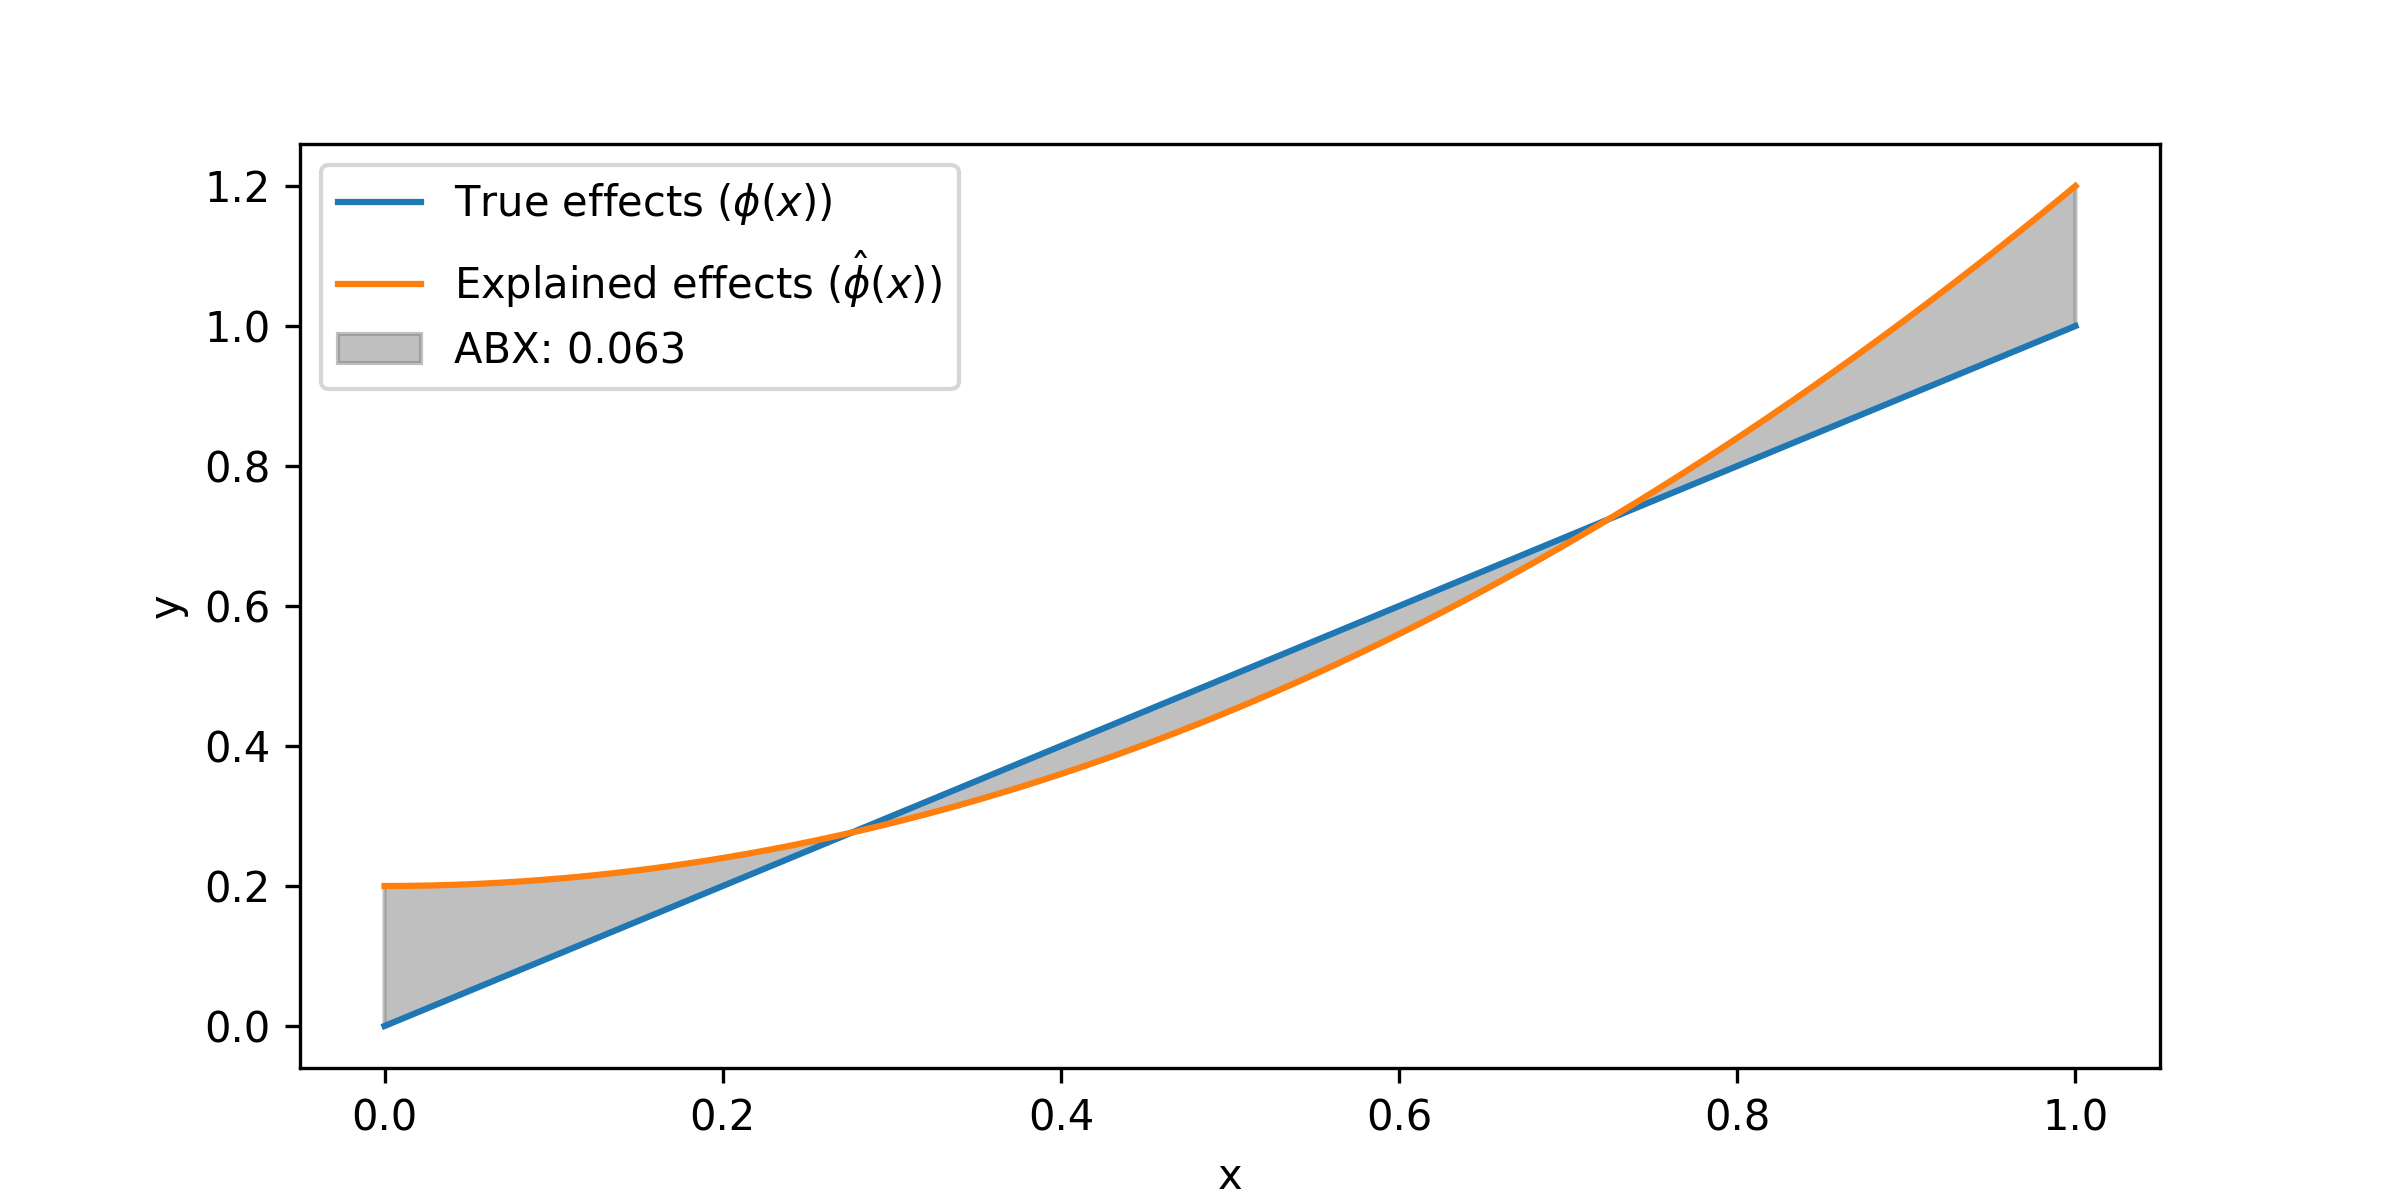
\includegraphics[width=0.7\textwidth]{images/extrapolation/area_example.png}}
\par\medskip\ABNTEXfontereduzida\selectfont%\textbf{Fonte:Elaborado pelo autor}  
\par\medskip
\end{figure}


\subsection{Experimental Setup}

Artificial data was used to provide a dataset where the true variable effects are known. Even in such a scenario, it is not guaranteed that the fitted function can recover the data-generating process, as discussed earlier in Section  \ref{xai_can_fail_but_is_usable}. To simplify the process for the predictive functions, simple scenarios were simulated. Specifically, four different datasets were created based on: $y^{i} = f(X^{i}) = X_{1}^{i} \cdot X_{2}^{i} + \epsilon_i$, where $\epsilon_i \sim N(0, 0.01)$. The variables $X_{1}$ and $X_{2}$ are dependent from the same uniform distribution $N(0,1)$ with the addition of a stochastic noise $N(0, 0.5)$. 

\begin{itemize}
    \item In the \textit{independent} scenario $y$ depends linearly only of $X_{1}$ and $f(X) = X_{1} + \epsilon$
    \item In the \textit{dependent linear scenario} $y$ depends linearly of both $X_{1}$ and $X_{2}$ being $f(X) = X_{1} + X_{2} \epsilon$
    \item In the \textit{first dependent non-linear} scenario $y$ depends linearly of $X_{1}$ and non-linearly of $X_{2}$ being  $f(X) = X_{1} + X_{2}^2 \epsilon$
    \item In the \textit{second dependent non-linear} scenario a more complex function was defined, and $y$ depends
    .linearly on $X_{1}$ and hold a non-linear cubic polynomial relationship with $X_{2}$ being  $y = x_1 + (x_2 - 0.9 x_2^3) + \epsilon$
\end{itemize}

All experiments were conducted within the R programming environment, utilizing a 30-Monte Carlo simulation framework to ensure robust statistical analysis. As discussed in Chapter \ref{chap2}, one of the primary models selected for data fitting in \gls{EDM} is the \gls{RF}, a choice motivated by its widespread acceptance and proven effectiveness in \gls{EDM} tasks. In addition to RF, we explored another algorithmic class often used in \gls{EDM} by incorporating a \gls{NN} model. Unlike the \gls{RF} model, which is characterized by piecewise constant functions potentially leading to more noticeable changes in model output with variations in input variables, the \gls{NN} model is based on differentiable functions, generally resulting in smoother transitions of output as input variables change. This contrast introduces greater diversity into our experimental design, allowing for a more comprehensive evaluation of post-hoc explanation techniques. 

The \gls{NN} was employed from the \textit{nnet} package\footnote{\url{https://cran.r-project.org/web/packages/nnet/index.html}}, and the RF from the \textit{randomForest} package\footnote{\url{https://cran.r-project.org/web/packages/randomForest/index.html}}. For each scenario, the number of sampled data points was varied with $N \in {200,500,1000}$. The parameters for the \gls{NN} algorithm—comprising ten nodes in the single hidden layer, a linear output activation function, and a regularization parameter of 0.0001—were determined to be approximately optimal through multiple iterations of 5-fold cross-validation for the first data scenario. The \gls{RF} algorithm was executed with default parameters.

To calculate the \gls{ABX} a numerical approximation was used. The approximation is based on the Trapezoidal Rule, implemented through the \textit{pracma}\footnote{\url{https://cran.r-project.org/web/packages/pracma/index.html}} package in R. This approach involves linearly interpolating between data points to form an approximate representation of the curve. The area under this curve is then estimated by dividing it into trapezoidal segments and summing their respective areas. 

Across all synthetic data scenarios, the average \gls{ABX} from the 30-Monte Carlo process was adopted as the final measure. To investigate the influence of the number of quantiles on the results, metrics were computed by dividing the data into quantiles with \(k=10\) and \(k=50\), where \(k\) represents the number of equally distributed parts.
